\documentclass{sigchi}

% Use this command to override the default ACM copyright statement (e.g. for preprints). 
% Consult the conference website for the camera-ready copyright statement.


%% EXAMPLE BEGIN -- HOW TO OVERRIDE THE DEFAULT COPYRIGHT STRIP -- (July 22, 2013 - Paul Baumann)
% \toappear{Permission to make digital or hard copies of all or part of this work for personal or classroom use is 	granted without fee provided that copies are not made or distributed for profit or commercial advantage and that copies bear this notice and the full citation on the first page. Copyrights for components of this work owned by others than ACM must be honored. Abstracting with credit is permitted. To copy otherwise, or republish, to post on servers or to redistribute to lists, requires prior specific permission and/or a fee. Request permissions from permissions@acm.org. \\
% {\emph{CHI'14}}, April 26--May 1, 2014, Toronto, Canada. \\
% Copyright \copyright~2014 ACM ISBN/14/04...\$15.00. \\
% DOI string from ACM form confirmation}
%% EXAMPLE END -- HOW TO OVERRIDE THE DEFAULT COPYRIGHT STRIP -- (July 22, 2013 - Paul Baumann)


% Arabic page numbers for submission. 
% Remove this line to eliminate page numbers for the camera ready copy
\pagenumbering{arabic}


% Load basic packages
\usepackage{balance}  % to better equalize the last page
\usepackage{graphics} % for EPS, load graphicx instead
\usepackage{graphicx}
\usepackage{times}    % comment if you want LaTeX's default font
\usepackage{url}      % llt: nicely formatted URLs
\usepackage[T1]{fontenc} 
\usepackage{subfigure}
\usepackage{balance}
\usepackage{url}
\usepackage{enumitem}
\usepackage{times}
%\usepackage{slashbox}
\usepackage{multirow}
\usepackage{color}
\usepackage{array}
\usepackage[table]{xcolor}
% http://ctan.org/pkg/xcolor   %{colortbl}
%\usepackage{slashbox}
\usepackage{colortbl}
\usepackage{color}
\definecolor{dark_green}{rgb}{0.2, 0.8, 0.0}
\definecolor{dark_yellow}{rgb}{0.9, 0.6, 0.1} %{0.6, 0.4, 0.2}
\usepackage{makecell}
\usepackage{tikz}


% llt: Define a global style for URLs, rather that the default one
\makeatletter
\def\url@leostyle{%
  \@ifundefined{selectfont}{\def\UrlFont{\sf}}{\def\UrlFont{\small\bf\ttfamily}}}
\makeatother
\urlstyle{leo}


% To make various LaTeX processors do the right thing with page size.
\def\pprw{8.5in}
\def\pprh{11in}
\special{papersize=\pprw,\pprh}
\setlength{\paperwidth}{\pprw}
\setlength{\paperheight}{\pprh}
\setlength{\pdfpagewidth}{\pprw}
\setlength{\pdfpageheight}{\pprh}

% Make sure hyperref comes last of your loaded packages, 
% to give it a fighting chance of not being over-written, 
% since its job is to redefine many LaTeX commands.
\usepackage[pdftex]{hyperref}
\hypersetup{
pdftitle={SIGCHI Conference Proceedings Format},
pdfauthor={LaTeX},
pdfkeywords={SIGCHI, proceedings, archival format},
bookmarksnumbered,
pdfstartview={FitH},
colorlinks,
citecolor=black,
filecolor=black,
linkcolor=black,
urlcolor=black,
breaklinks=true,
}

%\usepackage{ftnright}

% create a shortcut to typeset table headings
\newcommand\tabhead[1]{\small\textbf{#1}}
\newcommand{\vidya}[1]{\textcolor{red}{(vidya: #1)}}
\newenvironment{tight_itemize}{\begin{itemize} \itemsep
-2pt}{\end{itemize}}
\newenvironment{tight_enumerate}{\begin{enumerate} \itemsep
-2pt}{\end{enumerate}}


\toappear 

\teaser{
\centering
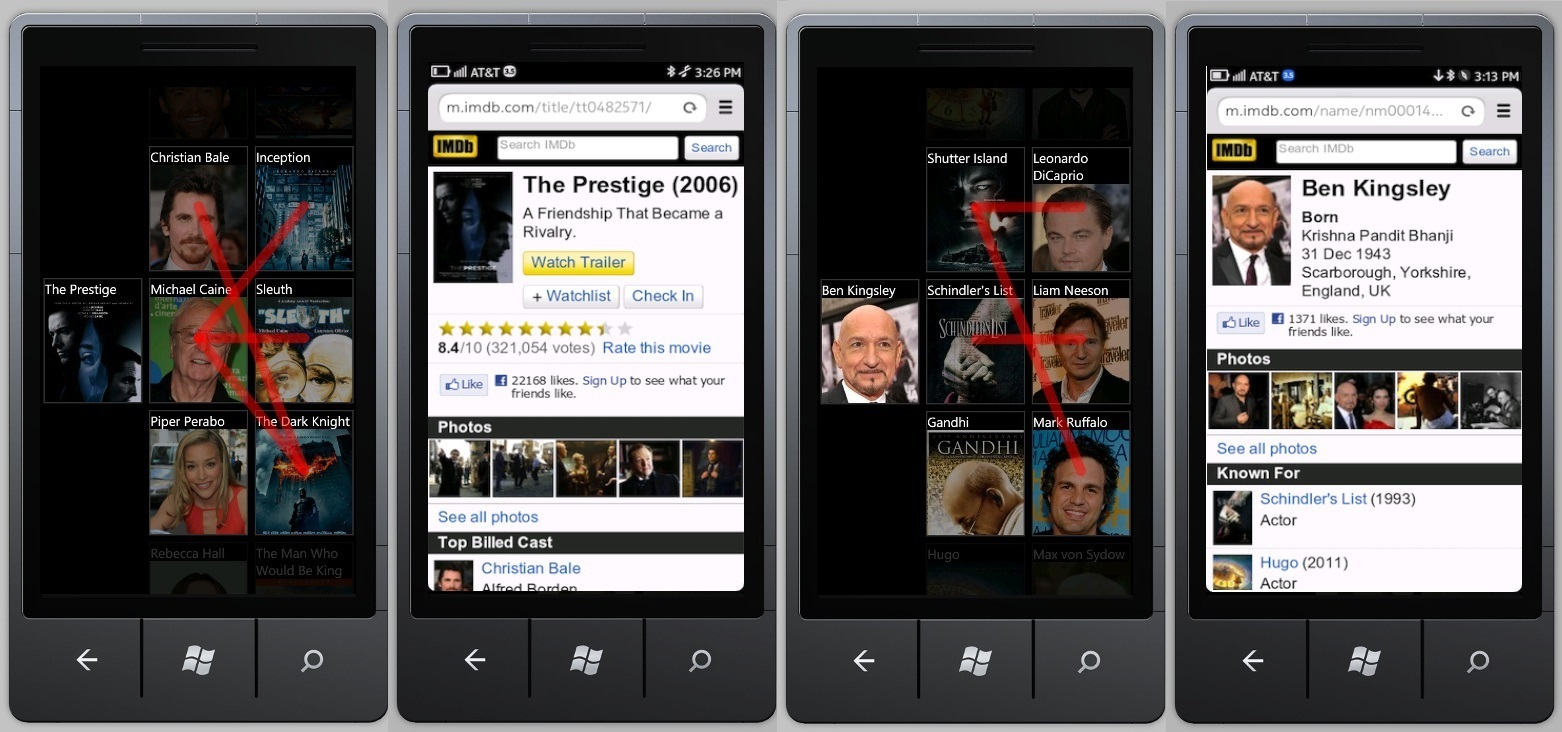
\includegraphics[width=7in]{images/teaser}
\caption{Comparing \textit{GraphTiles} with IMDb's mobile website. (a) and (b): The MPM(Movie-person-movie) \textit{QueryType}; (c) and (d): the PMP(Person-movie-person) \textit{QueryType}.}
\label{fig:teaser}
}



% End of preamble. Here it comes the document.
\begin{document}

\title{GraphTiles: A Visual Interface for Supporting \\Browsing and Imprecise Mobile Search}
%
%\numberofauthors{3}
%\author{
%  \alignauthor 1st Author Name\\
%    \affaddr{Affiliation}\\
%    \affaddr{Address}\\
%    \email{e-mail address}\\
%    \affaddr{Optional phone number}
%  \alignauthor 2nd Author Name\\
%    \affaddr{Affiliation}\\
%    \affaddr{Address}\\
%    \email{e-mail address}\\
%    \affaddr{Optional phone number}    
%  \alignauthor 3rd Author Name\\
%    \affaddr{Affiliation}\\
%    \affaddr{Address}\\
%    \email{e-mail address}\\
%    \affaddr{Optional phone number}
%}


\maketitle

\toappear

\begin{abstract}
Although mobiles are generating a rapidly increasing proportion of search queries, search interfaces have not changed significantly to accommodate mobile constraints. Imprecise search, which exists in the no-man's land between specific fact-finding and general browsing, is especially challenging in the mobile setting, when input is difficult and distractions complicate recall. We examined the prevalence of these mobile search use cases in a two-week diary study, finding that imprecise and general search accounted for the large majority of difficulty with search. Hypothesizing that the ability to view a link neighborhood around the search result could be quite helpful in these cases, we designed \textit{GraphTiles}, a visual interface for mobile search that exploits the structured entity relationships present in a significant portion of online datasets (e.g. IMDb~\cite{imdb} and LinkedIn~\cite{linkedin}). In an experimental evaluation, users found performed imprecise queries more quickly with \textit{GraphTiles} than with a standard mobile site. 
\end{abstract}
%I removed this example, seemed a bit week. Think we need one in the abstract? "For example, one user reported searching for the location where `The sisterhood of the traveling pants' was filmed. Although their search was successful, it was difficult. A visual overview of such relationships could have been very helpful. "

\keywords{
	 Mobile search, fact-finding, browsing, entity-relationship, imprecise queries.
	%\textcolor{red}{Mandatory section to be included in your final version.}
}


\category{H.5.m.}{Information Interfaces and Presentation (e.g. HCI)}{Miscellaneous}

%See: \url{http://www.acm.org/about/class/1998/}
%for more information and the full list of ACM classifiers
%and descriptors. 
%\textcolor{red}{Mandatory section to be included in your
%final version. On the submission page only the classifiers'
%letter-number combination will need to be entered.}






\section{Introduction}
\begin{figure*}[ht]
\centering
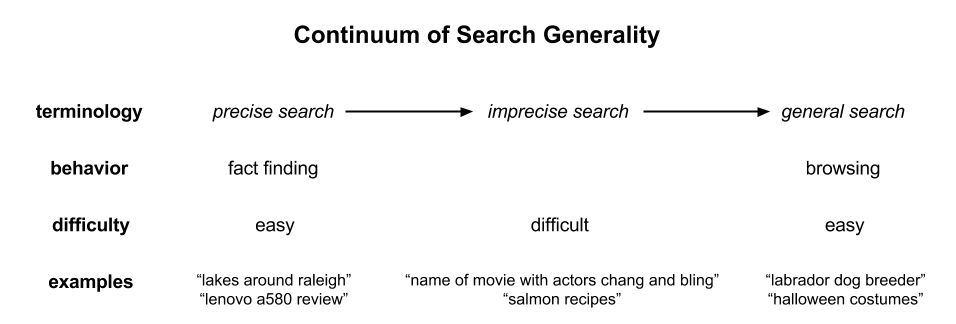
\includegraphics[width=\textwidth]{images/terminologydiagram}
\caption{ Our proposed continuum of search generality characterizes search according to the breadth of the information being sought. We expect that specific and broad information is generally easy for users to describe and find, but that this is not true with information in the ``no-man's land" between.}
\label{fig:searchcontinuum}
\end{figure*}




According to recent reports, mobile search will soon surpass desktop search as measured by both queries and ad revenue \cite{MobileQueries}\cite{MobileRevenue}. Despite this growing importance, Cui and Roto \cite{Cui:2008} and Church and Oliver \cite{Church:2011} find that current mobile search interfaces lead users to seek only information that is fairly specific (\textit{e.g.} fact-finding) or quite general (\textit{e.g.} browsing). Both types of information are easy to retrieve with queries, and easy to find in search results.

However, the lack of knowledge about the information they seek and the limited query capability of the mobile interface \cite{Kamvar:2009} can force mobile users to repeatedly reformulate their queries, and explore results extensively. For example, a user may seek a specific actor. If she cannot remember the name of the actor (in which case she would directly search by name), she might instead search for an actor who worked with the actor she is seeking. 

As Lee \textit{et al.} \cite{Lee:2012} point out, this ``no man's land" of \textit{imprecise} search (neither very general nor very specific) is more common than we might think, and some search engines have begun offering partial solutions. Search suggestions offer to complete keyword sets automatically in real time, helping users form better queries. Google's Knowledge Graph \cite{GoogleKnowledgeGraph} displays related facts from databases, making results easier to navigate; Yet neither solution is complete.

Inspired by this work, we propose a continuum of search generality from precise search to general search. It is based on the breadth of the information being sought, and is illustrated in Figure \ref{fig:searchcontinuum}.

We believe that we can improve imprecise mobile search further by exploiting the entity-relationship structure in many online information sources to give mobile users a better overview of their results. Such sources might include movies and cast in IMDb~\cite{imdb}, songs and artists in Pandora~\cite{pandora}, and friends in Facebook~\cite{Facebook}. These overviews reduce cognitive load through recognition, allow navigation of search results by attributes rather than only keyword \cite{Hearst:2002}, and guide users in the query reformulations that are typical of imprecise search.

In this paper, we present \textit{GraphTiles}, a visual search interface designed to help mobile users perform imprecise searches. The interface displays an incomplete portion of the local entity-relationship neighborhood: a thumbnail of the current page alone in the left column, some pages one link away in the middle column, and other pages two links away in the right column. 
%To see the complete neighborhood, users can scroll the central and right columns vertically. While this layout implies many links, it does not indicate exactly where the links are between the second and third columns. Users can reveal these locations by selecting a page thumbnail from these columns, triggering an \textit{interactive reordering} that highlights pages linked to the selection and places them onscreen or nearly so. Users can restore the original (better known) order by deselecting the page.


\section{Contributions}
The main contributions of this paper are:
\begin{itemize}
\item In a two-week diary study, we learned that most of the difficulty mobile search users experienced occurred during imprecise or general (browsing) searches.  
\item We designed the \textit{GraphTiles} system, supporting imprecise and general searches on mobile devices.
\item In a controlled experiment, we demonstrated that users were able to perform imprecise searches more quickly with \textit{GraphTiles} than with a standard mobile website.
\end{itemize}





\section{Related Work}

% Vidya: This is a repeat from the intro, so commented out.

%Mobile users often determine that finding information with mobile devices is more difficult than with desktop machines, and have adapted their use of mobile devices accordingly.
%Cui and Roto~\cite{Cui:2008} and Church and Oliver~\cite{Church:2011} found that mobile users effectively limit their expectations by posing either fairly specific queries or extremely broad ones. Browsing can easily satisfy open broad queries, while search can quickly answer very specific queries. Lee \textit{et al.}~\cite{Lee:2012} point out that human queries are often ill-formed and refined iteratively on the basis of intermediate query results. In a typical case, a user knows what they seek, but does not know the keyword that would retrieve it. Some search engines offer partial solutions by showing auto-completed keyword sets in real time (e.g. Bing's search suggestions), or by displaying related facts from a database (e.g. Google's Knowledge Graph). Even so, users are often forced to perform several searches to help them find the appropriate keywords for their search.

\textit{GraphTiles} exploits structured data sources to facilitate information discovery, and has similarities to faceted search and various category-based interfaces. There are several systems designed to support faceted navigation, allowing users to explore a collection of information by applying multiple classification filters. FaThumb supports navigation of a hierarchical information space by incremental text entry and attribute based filtering using a numeric keypad~\cite{Karlson:2006}. While text entry is fastest if one knows the specific information, facet navigation is faster when one only knows the attributes of that information. The MuZeeker application supports category based filtering to refine search by category selection rather than typing additional text~\cite{Larsen:2010}. The system uses contextual information from the search results to relate individual search results to external resources such as Youtube videos. mSpace Mobile employs fish-eyed multi-panes, where each pane returns information for a specific facet~\cite{mspace}.


One way of thinking about \textit{GraphTiles} is that it exploits knowledge of information locality to improve search. Similarly, other mobile search tools often take advantage of user context such as location and time to provide a localized experience. Lymberopoulos \textit{et al.} apply a data-driven approach where a local search model at different levels of location granularity (e.g. city, state, country) are combined together to improve click prediction accuracy in the search results \cite{Lymberopoulos:2011}. \textit{FindAll} is a local mobile search engine that lets users search and retrieve web pages, even in the absence of connectivity. The premise for their work is that mobile users often search for web pages that they have previously visited, known as re-finding. \textit{FindAll} estimates the benefits of local search, by learning the re-finding behavior of users~\cite{Balasubramanian:2012}. \textit{Hapori}, a local mobile search tool,  not only takes into account location in the search query but richer context such as the time, weather and the activity of the user~\cite{Lane:2010}. Amini \textit{et al.} present Trajectory-Aware Search (TAS) that predicts the user's destination based on location data from the current trip and shows search results near the predicted location~\cite{Amini:2012}. SocialSearchBrowser incorporates social networking capabilities with key mobile contexts to improve the search and information discovery experience of mobile users \cite{Church:2010}.

\textit{GraphTiles} is essentially a visualization of and search interface for the local entity-relationship graph. There has been little work specifically addressing mobile visualization ~\cite{RefWorks:658}, and to our knowledge, no work on mobile visualization for search. Karstens ~\cite{RefWorks:908} proposes node-link diagrams of hierarchies arranged around a rectangle to make efficient use of display space. He displayed nearly 1000 nodes, each represented with a very small circle. Hao and Zhang ~\cite{RefWorks:906} propose a space-filling sunburst display of hierarchies. Their larger nodes are easier to interact with, but their graphs are much smaller. Pattath \textit{et al.}  \cite{RefWorks:896} visualize general graphs numbering just a few dozen nodes using node-link diagrams. Finally, in work most closely related to our own, Da Lozzo \textit{et al.}\cite{springerlink:10.1007/978-3-642-18469-7-14} use node-link diagrams centered around a specific node, again with very small nodes. To recognize mobile constraints, \textit{GraphTiles} limits visualization to a graph neighborhood as do Da Lozzo \textit{et al.}, but like Hao and Zhang, it displays many links implicitly.


\section{Diary Study}
% Here is my plan for this section: 
% A) characterize the problem
% 1) define imprecise search as searches that require multiple queries (difficulty forming query) or multiple link following (difficulty navigating results) 
% 2) define difficult search as failed, rated difficult or taking a long time 

%Imprecise means 2 or more queries or 3 or more links clicked. 
%Too hard means failed, difficulty rating 4 or 5, or more than 2 minutes work. 

% 3) find how often imprecise happens, how often difficult happens, and whether difficult happens more often with imprecise 
% B) characterize a potential solution 
% 1) define structured data queries as search of known structured datasets or queries that could be answered by same 
% 2) find how often structured data queries happen, how often they intersect with imprecise and imprecise-difficult queries. 
% C) test hypotheses that 
% 1) imprecise queries are common enough todesign solutions for
% 2) imprecise queries are often difficult 
% 3) a solution for structured data queries would solve a significant portion of these 


\begin{table*}[ht]
\begin{center}
    \begin{tabular}{ | c | c | c | l |}
    \hline
    Category &  Number of Searches & Percentage & Query Examples \\ \hline
   \multirow{3}{*}{Precise and Easy} & & &  ``lakes around raleigh'' \\
    					   & 425 & 49 & ``data mining companies in the US''\\ 				
					   & &  &  ``lenovo a580 review''  \\ \hline 
					   
   \multirow{3}{*}{Precise and Difficult} & & & ``Where can I buy beautiful ruins at lowest price?'"\\
    					   & 61 & 7 & ``home remedy for cat diarrhea''\\ 				
					   & &  & ``how to transfer when taking a grey hound''  \\ \hline 

   \multirow{2}{*}{ Imprecise/General and Easy} & & & ``labrador dog breeder'"\\
    					   & 174 & 20 & ``flights to west coast''\\
					   & & & ``halloween costumes "\\ \hline 

   \multirow{2}{*}{ Imprecise/General and Difficult} & & & ``salmon recipes"\\
    					   & 208 & 24 & ``name of movie with actors chang and bling''\\
					   & & & ``bathroom vanity mirror, bathroom mirror"\\ \hline 

   
 \end{tabular}
\end{center}
\label{searchcategories}
\caption{Four categories of mobile searches in the diary study, their frequency of occurrence and examples.}
\end{table*}

We wanted to understand how often people perform \textit{imprecise} searches in regular use, and how searches influence difficulty. To capture mobile users outside of the lab, we opted for a two-week diary study, in which participants record their own behavior in their paper diaries, a technique similar to that used in \cite{Sohn:2008}. 

Imprecise searches can be characterized by at least one of two properties \cite{Lee:2012}:
\begin{tight_enumerate}
\item Users iteratively refine multiple queries to find relevant information due to difficulty formulating an exact query. 
\item Users have difficulty navigating through their search results to find the answer they are looking for, leading to multiple link following.
\end{tight_enumerate}

Accordingly we formulated the following definition of \textit{imprecise} search, as measured by our diary study: \textit{more than one query was required, or three or more links in the result list were followed}. However, we found one ambiguous case: one query and at least three followed links might be imprecise search, with a user arriving directly at a confusing set of search results and hunting around; or they might be general browsing search, with a user quickly finding a broad swath of interesting information, and slowly exploring it. Disambiguation might require knowing how rapidly users followed their links. Unfortunately, this sort of timing information is not reliable in diary studies. We therefore settled for grouping imprecise with general searches in our design. 

We now describe the participant profile, web diary tool, and procedure of our diary study.

\subsection{Participants}
We recruited $32$ participants ($21$ college students, $8$ software professionals, $2$ office secretaries, and $1$ school teacher) through online mailing lists and flyers. Their ages ranged between $18$ and $62$, with $17$ being male and $15$ female. All had normal or corrected-normal vision. They were required to have a mobile device capable of search, and to be regular users of that functionality. $14$ participants had iOS, $11$ had Android, and $7$ had Windows phones. 

\subsection{Procedure}
We provided each participant with a diary booklet to keep a history of their online searches. To keep the diary study agnostic across devices and the search medium, we opted for using a paper-based diary logging method as opposed to an automatic background logger. Participants were allowed to use any app or website on their device. Further, for privacy concerns, we wanted the participants to log only those searches that they were comfortable sharing. 

We asked them to record at least two searches per day in order to fill out a 25-page booklet over the two week period. We met each participant after a week in order to check their diaries and data, answer any questions, and help them improve their feedback. During the meeting, we audio-recorded the dialog to archive quotes and feedback. After the second week, we collected the booklets. Participants were either compensated \$9 or earned class credit. Each participant was assigned a unique ID to maintain their anonymity. If a participant completed a booklet before two weeks were over, we gave them a new one to fill out. We informed participants that they could terminate the experiment at any time, and that they should only divulge information that they were comfortable sharing. We also mentioned that we may publish anonymized quotes from their diaries. 

The booklet contained 25 pages and each page included the questions listed below. If participants were not able to find an appropriate answer, they provided an explanation. We asked the participants to write down these details as soon as possible after they performed a search. 

These were the questions on each page of the diary that participants answered as soon as they performed a search.
\begin{tight_enumerate}
            \item Date
            \item Time
            \item Duration of search task 
            \item What app or website did you access
            \item What were you searching for?
            \item Did you find what you were searching for at all? YES/NO
            \item If you did find your information, please continue by filling in the blanks with numbers: I performed \_ searches to find my information. I followed \_ links after leaving the search results page.
            \item Rate the difficulty of finding your information from 1--5 with 5 being very difficult. Add text to explain if you like.
\end{tight_enumerate}



\subsection{Results}

During the course of the diary study, we collected $868$ search entries with an average of 27 entries per person. 9\% of searches (33 out of 868) failed, not providing users with the information they sought. Participants performed an average of $1.2$ searches ($median=1, min =1, max=5$) and followed $2.5$ links ($median=2, min=0, max=39$) to find their information. Participants rated search difficulty at an average of $1.9$ ($median=2,  \sigma=1$). 

We categorized searches by type and difficulty. Searches were imprecise or general (browsing) when they employed more than one query or three or more links clicked in the result list. Otherwise, the searches were precise (fact finding). Searches were too hard when they failed, users rated them difficult ($4$ or $5$ on the scale), or they required more than $2$ minutes of searching. Otherwise, searches were easy. 

Using these two categories, we were able to bin the searches into four combined groups. 49 \% of the searches were precise and easy, 7 \% were precise and difficult, 20 \% were imprecise or general and easy, and 24 \% were imprecise or general and difficult. 

Although search was usually successful, it was difficult about a third of the time (31\%), especially when search was more imprecise or general. In fact these searches formed the large majority of the difficulties users were having. Further, roughly one third of imprecise and general searches sought information from datasets structured by entity relationships, such as movies and crews (\url{www.imdb.com}) or recipe ingredients and dishes (\url{allrecipes.com}). (This number may be significantly larger, because many participants only recorded their search tool, not the information they sought).

Some of the comments by the study participants on why they found imprecise or general searches to be difficult, include: \textit{``could not come with the right descriptors for the mirror to find the one I had seen in the store"}, \textit{``had to navigate lots of links to find something useful"} , \textit{``had a hard time finding the right video of the musician as I didn't remember his name"}, \textit{``could not come up with the right search terms to find a book by a particular author and did not remember the author"}. Table 1 shows various corresponding examples.

On reflection, it is not surprising that search difficulty was focused in imprecise or general task types: they are simply more complex. We believe the large majority of problem searches could have benefited from a tool that helped users navigate through the complex information neighborhoods typical of imprecise and general search, and that a good starting point for such a tool would be exploiting the structure available in many datasets. 

% Vidya: I don't think these two paras are relevant to this paper. Ben: agreed.

%The average time taken to record a search activity was $131.6$ seconds ($median=120, max=1200$). 
%People use applications more than websites for certain activities. On an average, 18.5\% (160 out of 868) of the searches were using applications than web portals. The most popular category searched using an application was \emph{shopping} (47\%). Surprisingly, participants frequently knew the exact keyword to put in as a search phrase. People use mobile apps for regular, standard search activities (i.e. weather, shopping, location, names, exchange rate, bus route, definition). For less frequent, more complicated searches, they will try it on a web portal but easily give up because of the screen size restriction and choose another method (i.e. go to their desktop, ask friends).

%
%We looked for duplicate themes from collected diary entries and did not start with a set of fixed categories. We adopted most of the categories from \cite{chi2008} and added new categories such as `\emph{how-to}', `\emph{unit conversion}', `\emph{definition}', and `\emph{name}'. There are 17 categories based on the diary entries.
%The \emph{how-to} category includes information about practical advice and detailed instruction of an activity. The \emph{unit conversion} includes kilometer to miles conversion, fahrenheit to celsius, and exchange rate. The \emph{definition} includes any need of terminology definition and detailed explanation. The \emph{name} includes search of a certain person or movie title. The largest category of collected entries was \emph{trivia} (51\%). They are the random thoughts from the participants such as ``story of shutter island". The second highest was \emph{shopping} (13\%), followed by \emph{point of interest} (10\%) and \emph{definition} (6\%).



%Vidya: I think this figure is hard to understand and looks too complicated. Ben: agreed.
%Figure \ref{fig:searchtype} categorizes search type of diary entries by success/failure, easy/difficult, open/specific queries, and hit or miss. Overall, the large blue section shows that people are mostly successful in finding information with their mobile device (though they may never attempt many challenging searches). About a third of searches are still difficult, and over half of difficult searches are open. 
%
%
%\begin{figure}[ht]
%\centering
%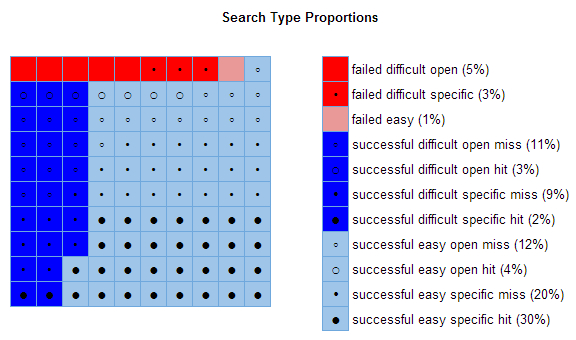
\includegraphics[width=3in]{images/searchtype}
%\caption{Search type by success/failure, easy/difficult, open/specific, and hit/miss. Blue: success, red: failure, saturated color: easy, bright color: difficult, empty dot: open, filled dot: specific, smaller dot: miss, bigger dot: hit}
%\label{fig:searchtype}
%\end{figure}







\section{The GraphTiles interface}
We designed \textit{GraphTiles} to help mobile search users handle the most challenging use case identified by our diary study: general or imprecise search. With general search, users browse and cast a wide net. We expected a tool providing a good overview of search results to help them find the most interesting results. With imprecise search, users have difficulty characterizing their search, typically reformulating their queries and exploring intermediate results to hone in on and find reminders of what they seek. Again we expected a visual overview to aid users. \textit{GraphTiles} exploits the structure available in many online datasets to produce this overview. 

With \textit{GraphTiles} (Figure \ref{fig:teaser} (a),(c)), we assume that users will employ search to find a locality of concern around a central node (e.g. for IMDb, ``near John Wayne"), represented by a thumbnail alone in the left column. Distance in the \textit{GraphTiles} layout from this central node reflects relational distance from the center (e.g. for IMDb, degrees of working separation from John Wayne), with the middle column one link away, and the right column two links away. To see the complete two link neighborhood, users can scroll the central and right columns vertically. We display links largely implicitly: every node in the middle column has an implied link to the central node, and every node in the right column is reachable from the middle column. To represent links between the middle and right columns we support both explicit link display, and interactive reordering. Explicit links appear only when both linked nodes are currently displayed. With reordering, when users select a thumbnail from these columns, \textit{GraphTiles} highlights thumbnails linked to the selection and reorders to place them onscreen or nearly so. Users can restore the previous order by deslected the thumbnail. When necessary, users can drag a non-central node to the left to change the central node.

We considered a circular (or rectangular) layout to make better use of the blank space in the left column, with a scroll around the central node rather than along it, but discarded it so that we could provide a glimpse of a larger two-link neighborhood. A circular layout with a two-link neighborhood would require much smaller nodes (difficult to touch with a finger tip), and would fit poorly in rectangular mobile displays. Representing within column links explicitly can be confusing, so for such cases we rely on interactive reordering alone (see (c) in Figure \ref{fig:musicband}, depicting data from the Seattle Band Map ~\cite{seattleband}).


\section{Experiment: Comparison to IMDb's Mobile Site}
\begin{figure*}[t]
\centering
\subfigure[Band and artist relationship]{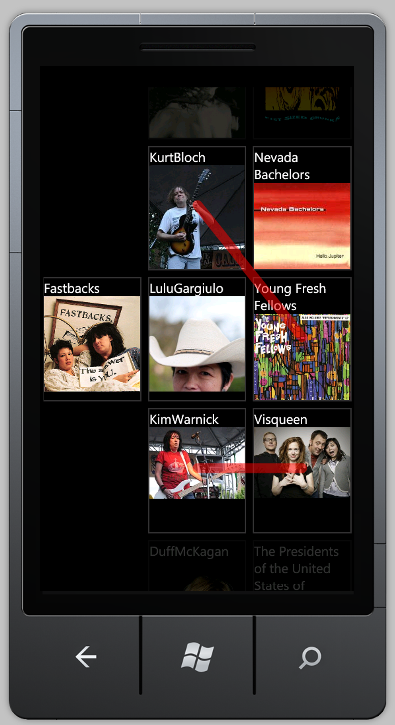
\includegraphics[width=1.6in]{images/bab}}
\subfigure[Band relationship]{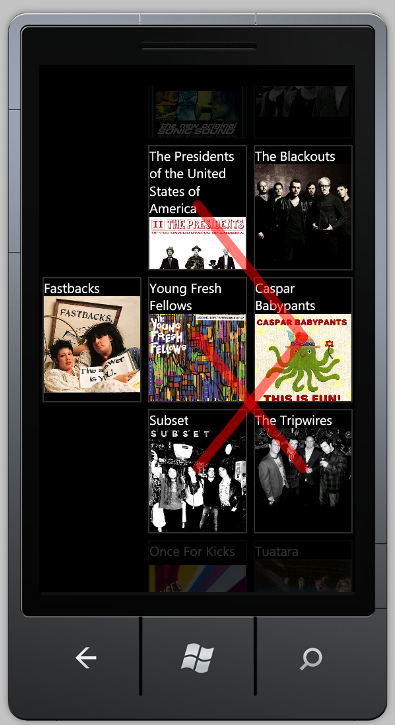
\includegraphics[width=1.6in]{images/bbb}}
\subfigure[Interactive reordering with dimmed image when not related.]{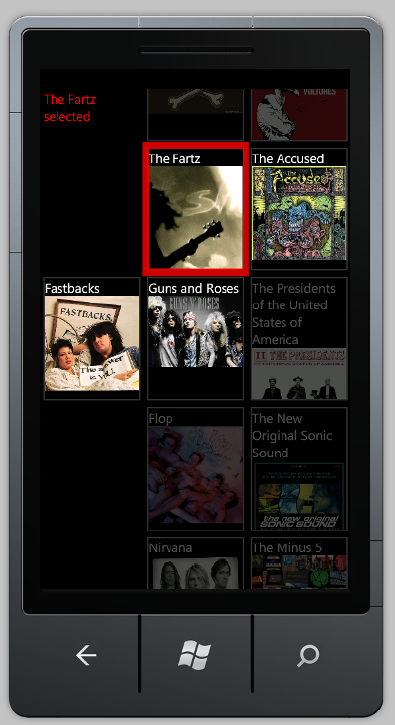
\includegraphics[width=1.6in]{images/fartz_reordering}}
\caption{Applying \textit{GraphTiles} to Seattle's music band data.}
\label{fig:musicband}
\end{figure*}


To confirm that \textit{GraphTiles} supported imprecise search well, we performed an experiment comparing it to a standard mobile information interface. We expected that the specialized \textit{GraphTiles} interface would allow users to perform imprecise search more quickly than an interface supporting the full continuum of information-seeking.

As a typical mobile information interface, we chose the IMDb mobile web app. An imprecise search making use of IMDb is often similar to this: a user wants to recommend a movie to a friend, but cannot remember the name of that movie, nor the name of any actors in that movie. This makes using standard search interfaces somewhat difficult. They do however know that one of the actors in the movie they want to recommend was also in a different movie they can name. They navigate from movie to actor to movie. We focused on answering imprecise queries of that nature. 

Figure \ref{fig:teaser} shows a comparison of the visuals used in \textit{GraphTiles} and IMDb's mobile website (\url{http://m.imdb.com}) to answer movie-person-movie(MPM) queries of this type, as well as person-movie-person(PMP) \textit{QueryTypes}.


\subsection{Method}

Our experiment had $20$ participants, all of them employees at a large corporate research center.  We obtained informed consent from the participants, and asked them to read the instructions for the experiment. We then familiarized them with the task using 8 training datasets, two for each combination of link \textit{interface} and \textit{QueryType}. Participants were free to ask verbal questions during training. Each participant performed $120$ information seeking tasks, each using a different graph neighborhood in the IMDb database, with median size of 115 nodes. On average, they completed all their tasks in one hour.

We used a fully crossed within subjects $2 \times 2$ design. As participants performed the tasks, we systematically altered two variables. \textit{Interface}, or the tool used to access the IMDb information, had two levels: \textit{GraphTiles} and the IMDb web app. \textit{QueryType} had two levels: a movie-person-movie (MPM) query or a person-movie-person (PMP) query. If \textit{QueryType} was MPM, we asked participants to find the person who worked in two given movies. In this case, the central node at the left of the visualization was always a movie. If \textit{QueryType} was PMP, we asked participants to find the movie on which two given people collaborated. In this case, the central node at the left of the visualization was always a person. 

To answer a question, participants typically scrolled in the right column to find the second given person or movie. This reordered the middle column, making it easier to scroll in the middle column to find and select the connecting movie or person. Alternatively, participants could first scroll in the middle column, then select each movie or person there and scroll the reordered right column to find the second given person or movie. However, participants quickly learned that the right-first approach was more efficient: it took advantage of faceted search to require only one switch between the right and middle columns, while the middle-first approach ignored the provided faceted search parameter and required several switches.

\textit{GraphTiles} displayed link lines and used interactive reordering. Every participant performed $30$ trials with each of the $2 \times 2 = 4$ experimental treatments. We grouped trials by \textit{Interface} into two blocks of $60$ trials each. Thus participants performed all trials with the current Interface before moving on to the next. To combat the effects of fatigue and learning, we used complete counterbalancing across participants: half of them performed the \textit{GraphTiles} block first, the other half the web app block first. Within each of these blocks, we randomly ordered the levels of \textit{QueryType}. We randomized the order of graph neighborhoods without replacement, so that each participant saw each neighborhood exactly once.

\subsubsection{Apparatus}

We implemented \textit{GraphTiles} on three Samsung SGH-i917 phones running Windows Phone 7.5, with an AMOLED display and a full capacitive touch screen. The monitor used to display questions was a $1920 \times 1200$ pixel Dell 24''. Participants interacted with the visualization on a phone by scrolling with a swipe gesture or selecting nodes with a long tap.

We obtained our IMDb graph neighborhoods using the official IMDb API (\url{http://www.imdb.com/interfaces}), obtaining a large cross section of its database (approximately 3GB in size). We then randomly selected 60 nodes within the IMDb graph describing well known actors (supporting PMP queries), and 60 nodes describing well known movies (supporting MPM queries). We then sampled the two-link neighborhood around each actor (PMP) node by adding the top movies linked to it as indicated by IMDb's own API call; and then for each of those top movies, adding its top actors, again as indicated by IMDb's API call. We created two-link neighborhoods around movie (MPM) nodes similarly. The number of top movies returned by IMDb's API was generally much lower than the number of top actors. 


\subsection{Results}

All participants performed all trials correctly, so we report only completion times here. We tested significance using a two-factor repeated measures ANOVA. Only the two single variable effects were significant; they did not interact. 

When using \textit{GraphTiles}, participants were significantly ($F(1,19)=2291.833$, $p<0.001$) faster than when using the IMDb web app. Average completion time with \textit{GraphTiles} was 18.2s ($\sigma =5.27$), while with IMDb web app, it was 31.5s (SD 5.26).

Although its effect was significant ($F(1,19)=11.27$, $p<0.005$), \textit{QueryType}'s effect was not meaningful. The difference in completion times when participants looked for movies rather than persons was 0.6s: (25.0s for movies, 24.4s for persons). The likely explanation for this effect was the consistent differences in MPM vs. PMP neighborhoods.


\subsection{Discussion}

Results in fact exceeded our expectations, with \textit{GraphTiles} users almost twice as fast as IMDb web app users. There are two explanations for \textit{GraphTiles}'s superior performance. First and most important, the faceted search implemented in \textit{GraphTiles} reduced the number of actions users had to take. By first selecting both given people or movies, users could display only the movies or people connecting them. In contrast, IMDb did not implemented faceted search, and required users to examine a much larger set of possibly connecting movies or people. Second, \textit{GraphTiles} had several visual advantages. It was a more effective overview: rather than requiring interaction to reveal information two links away (i.e. other people in the first person's movies, or other movies in which the cast of the first movie acted), it displayed at least some of them immediately. \textit{GraphTiles} was also less cluttered, without the ads and tertiary information IMDb contains. Finally, \textit{GraphTiles} was less textual than IMDb, and perceptual research consistently shows that visual information is more rapidly understood than text.

Although the degree of \texit{GraphTiles}'s superiority was surprising, that superiority itself was not. \textit{GraphTiles} was designed specifically for imprecise search; IMDb is a more general tool. What remains to be seen is whether or not a single interface can support the full continuum of search generality well. Future work might also attempt to extend our results with other and more types of imprecise search, and by examining the performance of \textit{GraphTiles} with general and indeed precise search.


% Ben: don't think we need to belabor this point. Taking it out.
%\section{GraphTiles in Non-bipartite Graphs}
%While real and practical, the IMDb graph is bipartite: nodes contain two disjoint sets of either people (e.g. actors) or movies. \textit{GraphTiles} quite appropriately exploits this structure, placing people and movies in different columns. However if \textit{GraphTiles} is to find use with more general applications, it must be tested with non-bipartite graphs. 

With this goal in mind, we used \textit{GraphTiles} to the Seattle Band Map . In this database, music bands from the Pacific Northwest are linked if they share band members or have collaborated with one another. By preprocessing the database, we could create a bipartite graph of musicians and bands where musicians and bands (Figure \ref{fig:musicband}(a)), but that is not our purpose here. 

Figure (b) shows a non-bipartite band-band layout using lines to represent links. The challenge here is representing links that start and end within the same \textit{GraphTiles} column, which do not exist in bipartite graphs. Lines and most of the other explicit link representations we discussed perform poorly in such cases, since they are only displayed when both endpoints are onscreen, which will happen only rarely within the same column.

We believe interactive reordering is the best solution to this problem. In Figure \ref{fig:musicband}(c), the user selects the band `The Fartz', bringing all related bands onscreen or nearly so. Unrelated bands are dimmed out in the interface to further accentuate band connections.




% Ben: not an important contribution. Removing this.
%\section{Experiment: Comparison of Explicit Link Representations}
%We considered how to display links explicitly on the mobile screen. It might be tempting simply to draw lines between linked nodes (Figure \ref{fig:linkrep}c), but \textit{GraphTiles} has unique characteristics that could make this solution untenable. As users scroll, nodes appear and disappear, meaning that linking lines do as well. Scrolling also causes the lines to move when they are onscreen, occluding a variety of other nodes and dynamically relocating link crossings (making a well-known drawback of link lines still worse). All of this dynamic behavior does not exist in most graph visualizations and could be quite disorienting during mobile search. .

In creating alternative designs for displaying explicit links, we were (loosely) inspired by the grouping principles of Gestalt psychology ~\cite{RefWorks:562}. The \textit{proximity} principle places nearby items in the same group. Because we could not use proximity alone to display complex many-to-many relationships, we approximated proximity with an iconic representation of the neighboring column (Figure \ref{fig:linkrep}(d)). Rectangles in the representation indicate the presence of links to the node in the same position in the neighboring column. \textit{Similarity} groups items that have similar properties such as color or texture (Figure \ref{fig:linkrep}(b) and \ref{fig:linkrep}(e)). Here, nodes containing the outline color or a thumbnail of a neighboring node are linked to that node. Like link lines (which use the Gestalt principle of \textit{connectedness}), all of these representations must dynamically change as the user scrolls and nodes move, but the changes are much more restrained.

\begin{figure*}[htb!]
\centering
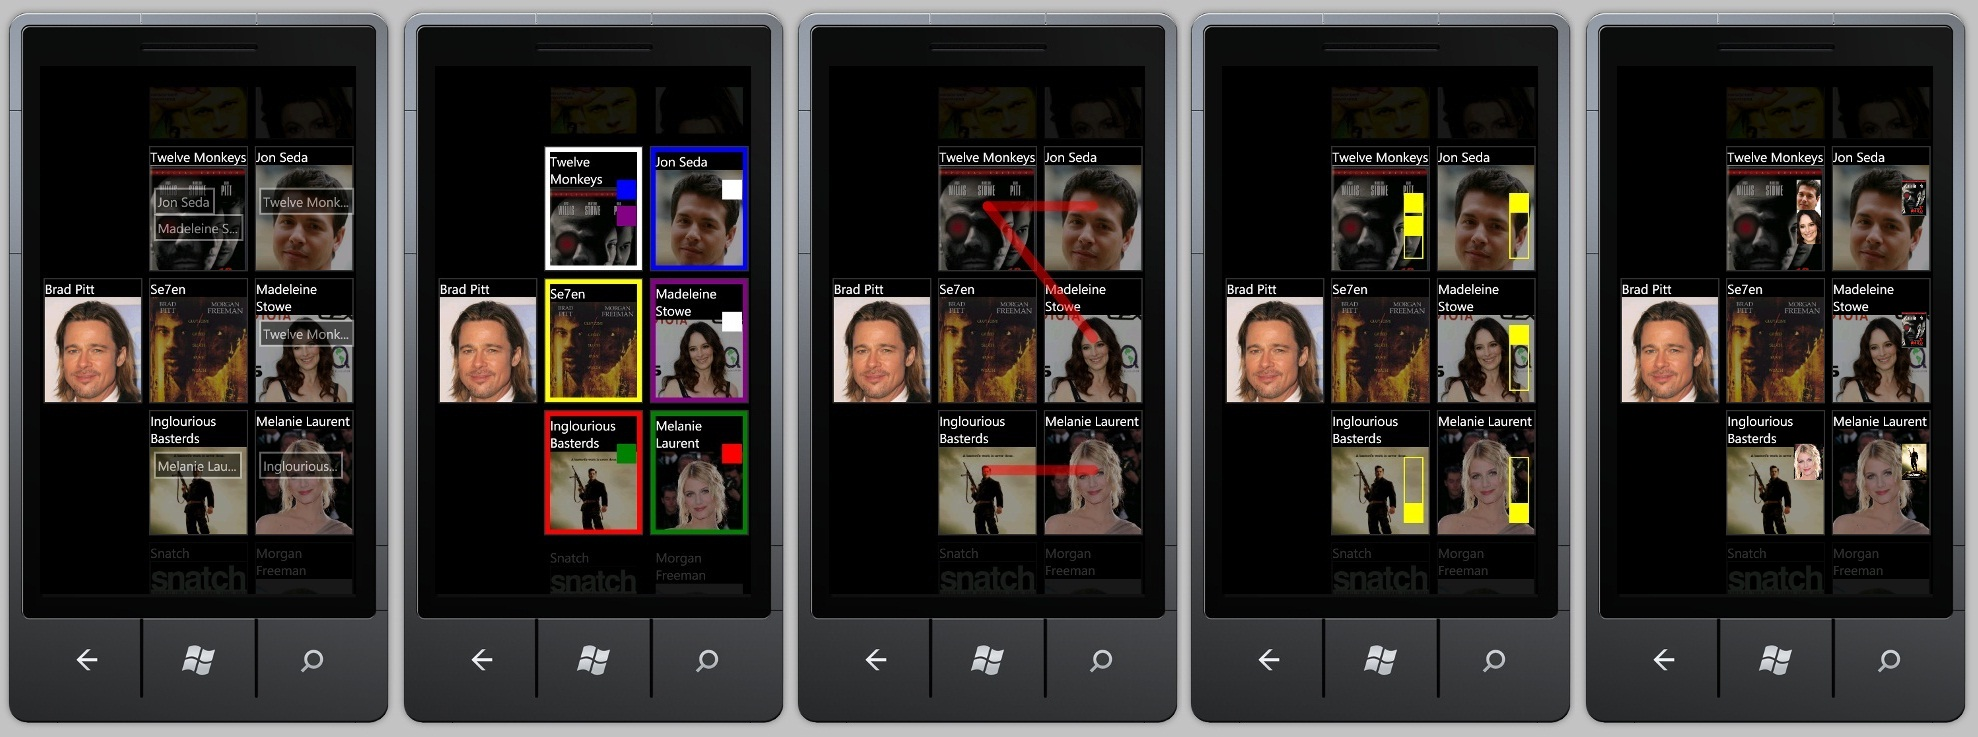
\includegraphics[width=7in]{images/linkrep}
\caption{Different explicit link representations for \textit{GraphTiles}. (a) \emph{text:} nodes with the same name are linked. (b) \emph{color:} nodes with the same color are linked. (c) \emph{connectedness:} nodes with lines between them are linked. (d) \emph{proximity:} nodes at/containing the same vertical position are linked. (e) \emph{texture:} nodes with/containing the same image are linked.}
\label{fig:linkrep}
\end{figure*}

\subsection{Method}

Using IMDb as a testbed, we compared connectedness-inspired lines to our alternative designs in a controlled experiment, and included a text-based link display (Figure \ref{fig:linkrep}(a)) as a control condition. In this condition, nodes with the same text were linked. Note that because we were testing only explicit link representations, we did not enable interactive reordering in this experiment.

We expected that connectedness-, color- and texture-inspired links would perform better than text-based or proximity-inspired links. Because of the unique dynamic qualities of the \textit{GraphTiles} visualization, we did not attempt to predict which link representation would be best.

\subsubsection{Design}

We used a fully crossed within subjects $5 \times 2 \times 2$ design. Link \textit{Depiction} had five levels: text-based as well as proximity-, color-, texture-, and connectedness-inspired representations. \textit{QueryType}, or the type of question asked, had two levels: a movie-person-movie (MPM) query or a person-movie-person (PMP) query. \textit{Size}, or the rough size of the surrounding graph neighborhood, had two levels: small or below median, and large or above median.


\subsubsection{Participants and Procedure}

We had ten participants, all university students with normal or corrected-to-normal vision. We obtained informed consent from the participants, and asked them to read the instructions for the experiment. We then familiarized them with the task and link depictions using 10 training datasets, one for each combination of link \textit{Depiction} and \textit{QueryType}. Participants were free to ask verbal questions during training.

Participants then each performed $120$ information seeking tasks, each using a different graph neighborhood in the IMDb database, with median size of 115 nodes. On average, they completed all their tasks in one hour. Every participant performed six trials with each of the $5 \times 2 \times 2 = 20$ experimental treatments. We formed five blocks of $24$ trials each, each block corresponding to one \textit{Depiction}. Thus participants performed all trials with the current \textit{Depiction} before moving on to the next. To combat the effects of fatigue and learning, we sampled all the orderings of \textit{Depiction} using a $5 \times 5$ Latin Square. Within each of these \textit{Depiction} blocks, we formed two 12-trial \textit{QueryType} blocks. Half of the participants performed MPM questions first, half performed PMP questions first. Within each \textit{QueryType} block, participants performed 6 trials with small neighborhoods and 6 with large neighborhoods. We randomized the order of these trials. To avoid any confound between treatments and graph neighborhoods, we randomized the match of graph to treatment. Each participant saw each neighborhood only once.

For each task, participants answered a question displayed on a nearby monitor. 
As for the \textit{QueryType}, we used the same method as the previous summative experiment.
We recorded the time to complete each trial, and whether or not the participant performed the trial correctly. Participants were paid \$10 for their effort.


\subsection{Results}
\begin{figure}[ht]
\centering
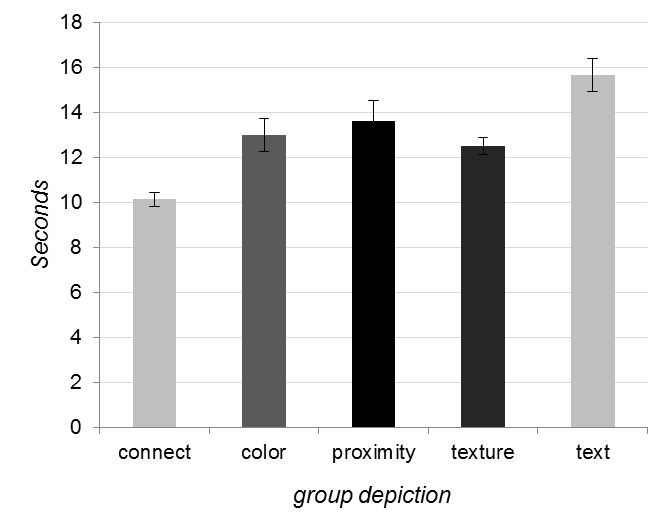
\includegraphics[width=3in]{images/depictiongraph}
\caption{Average task completion times per depiction for the first experiment.}
\label{fig:experiment1}
\end{figure}

All participants completed all trials correctly, so we report only on completion time here. On completion times, we performed a single, three-factor repeated measures ANOVA. All single variable effects were significant. 

The connectedness-inspired link Depiction indeed supported the fastest information seeking performance ($F(4,36)=4.942, p<0.005$). Average completion times in seconds for each Depiction were: connectedness $10.1$s, texture $12.5$s, color $13.0$s, proximity $13.6$s, and text $15.7$s. We show the same times in Figure \ref{fig:experiment1}, along with standard error. Despite their drawbacks, link lines also have strengths: they are familiar to most viewers;  and they are simple, introducing only one primitive per link, while other representations require changes at both linked nodes.


Participants were much faster when asked to locate a person (the MPM \textit{QueryType}) than when asked to locate a movie (PMP) ($F(1,9)=43.869, p<0.001$). Average completion times for person queries were 10.5s, and for movies 15.5s. This is likely an effect of graph size rather than some more subtle task difference. Recall that IMDb's API returned many more top actors working on a movie than top movies in which an actor worked. This meant that PMP neighborhoods contained many more nodes than MPM neighborhoods.

Participants were faster when working with small graph Sizes than with large graph Sizes ($F(1,9)=83.911, p<0.001$). Average completion times for small graphs were $11.7$s, while for large graphs they were $14.2$s.

The only significant interaction occurred between the \textit{QueryType} and \textit{Size} variables ($F(1,9)=25.824, p=0.001$). When participants were asked to find movies in PMP neighborhoods, increasing graph Size had a large effect on completion times ($13.4$s vs. $17.6$s). When they were asked to find persons in MPM neighborhoods, \textit{Size}'s effect was minor ($10.1$s vs. $10.9$s). In PMP neighborhoods, graphs were larger, so increasing \textit{Size} had a larger effect.

Readers may wonder why average times in this experiment with \textit{GraphTiles} were lesser than they were in our first experiment. One cause may be the increased practice with \textit{GraphTiles} (10 training datasets) in this experiment.


\subsection{Discussion}
Results largely matched our expectations, with text-based and proximity-inspired links performing worst, texture- and color- inspired link \textit{Depictions} performing better, and connectedness-inspired link lines performing best. However, users were only about 20\% faster with link lines than with texture-inspired links containing thumbnails.





\section{Conclusion and Future Work}
As mobile devices become the dominant form of computing, mobile search will become increasingly important. In this paper we described \textit{GraphTiles}, a new search interface specifically designed for general browsing and imprecise search. In a diary study, these more complex types of search proved to be the focus of most user difficulty. In an experimental evaluation, accessing the IMDb graph for imprecise search with \textit{GraphTiles} was nearly twice as fast as with the existing IMDb mobile web app.

A number of possible design improvements to \textit{GraphTiles} could be studied in future work. The current design is optimized for smartphones; on devices such as tablets \textit{GraphTiles} might display larger neighborhoods. \textit{GraphTiles} could also use improvements to maintain visual continuity when users change the central node: currently users can quickly become disoriented. 

Several limitations and open questions in our work also deserve followup. How easily could \textit{GraphTiles} be generalized?  There are two primary data constraints that we exploited in \textit{GraphTiles}. First, the presence of visual thumbnails, which are an effective way of improving experience and summarizing available information~\cite{Setlur:2011}. Second, the existence of a structuring graph of entities and their relationships, which enable users to navigate through information in an intuitive manner. In our experience, there are many sites that match these constraints, including IMDb~\cite{imdb}, AllMusic~\cite{allmusic} and Allrecipes~\cite{allrecipes}. 

With imprecise and difficult queries such as ``salmon recipes" and ``bathroom mirror" shown in Table 1, one could substitute text for the thumbnails. For example, the GraphTiles interface could initially display abridged ingredients of salmon dishes with additional interaction for showing longer descriptions. Another option is to show summarized thumbnails containing both text and imagery. While it remains to be seen how effective this would be, a navigable structure is a necessity. It may be possible to use the links in a webpage or search engine results to provide this structure.

Will or should \textit{GraphTiles} always be a special case, or can it be part of a unified solution for specific as well as imprecise and general search? Finally, it could be profitable to learn about the various contributions to mobile search difficulty of general vs. imprecise search. We were not able to disentangle the two in the diary study we used here, but future work might employ a different measurement method.



%\begin{table}[h]
%\centering
%\begin{center} {\footnotesize
%{\renewcommand{\arraystretch}{1.2}%
%\begin{tabular}{|l||l|}
%\hline
%\textbf{independent variable}  &  \textbf{ANOVA of time} \\
%\hline
% &     F(,)=, p= \\
%\hline
%\end{tabular} }} \quad
%\end{center}
%\caption{\footnotesize Significant main effects on time.}
%\label{table:timeAnova}
%\end{table}
%\balance

% Balancing columns in a ref list is a bit of a pain because you
% either use a hack like flushend or balance, or manually insert
% a column break.  http://www.tex.ac.uk/cgi-bin/texfaq2html?label=balance
% multicols doesn't work because we're already in two-column mode,
% and flushend isn't awesome, so I choose balance.  See this
% for more info: http://cs.brown.edu/system/software/latex/doc/balance.pdf
%
% Note that in a perfect world balance wants to be in the first
% column of the last page.
%
% If balance doesn't work for you, you can remove that and
% hard-code a column break into the bbl file right before you
% submit:
%
% http://stackoverflow.com/questions/2149854/how-to-manually-equalize-columns-
% in-an-ieee-paper-if-using-bibtex
%
% Or, just remove \balance and give up on balancing the last page.
%
%\balance

\bibliographystyle{acm-sigchi}
\bibliography{sample}
\end{document}
